\section{Simplicial Abelian Groups}
\label{sec:Simplicial Abelian Groups}

Before defining \emph{simplicial abelian groups}, we will first discuss the more general notion of \emph{simplicial sets}. There are generally two definitions of simplicial sets, an abstract one and a very explicit one. We will start with the abstract one, luckily it can still be visualised in pictures, then we will derive the explicit definition. The reader who is interested in how these notions are developed, should consider reading the introduction by Friedman \cite{friedman}, which also gives nice illustrations.

\subsection{Abstract definition}
\begin{definition}
	We define a category $\DELTA$, where the objects are the finite ordinals $[n] = \{0 < \dots < n\}$ for $n \in \N$ and maps are monotone functions: $\Hom{\DELTA}{[n]}{[m]} = \{ f : [n] \to [m] \I f(i) \leq f(j) \text{ for all } i < j \}$.
\end{definition}

The category $\DELTA$ is sometimes referred to as the \emph{category of finite ordinals} or the \emph{cosimplicial index category}. There are two special kinds of maps in $\DELTA$, the so called \emph{face} maps and \emph{degeneracy} maps. The \emph{$i$-th face maps} $\delta_i: [n-1] \to [n]$ is the unique injective monotone function which \emph{omits} $i$. More precisely, it is defined for all $n \in \Np$ as (note that we do not explicitly denote $n$ in this notation)
$$ \delta_i: [n-1] \to [n], k \mapsto \begin{cases} k & \text{if } k < i,\\ k+1 & \text{if } k \geq i, \end{cases} \hspace{1.0cm} 0 \leq i \leq n. $$

The \emph{$i$-th degeneracy map} $\sigma_i: [n+1] \to [n]$ is the unique surjective monotone function which \emph{hits $i$ twice}. More precisely it is defined for all $n \in \N$ as
$$ \sigma_i: [n+1] \to [n], k \mapsto \begin{cases} k & \text{if } k \leq i,\\ k-1 & \text{if } k > i, \end{cases} \hspace{1.0cm} 0 \leq i \leq n. $$

The nice things about these maps is that every map in $\DELTA$ can be decomposed to a composition of such maps. So in a sense, these are all the maps we need to consider.

\begin{lemma}\emph{(Epi-mono factorization)}
	\label{le:epimono}
	Let $\eta : [m] \to [n]$ be a map in $\DELTA$. Then $\eta$ can be uniquely decomposed as
	$$ \eta = \delta_{i_a} \cdots \delta_{i_1} \sigma_{j_b} \cdots \sigma_{j_1}, $$
	such that $0 \leq j_b < \cdots < j_1 < m$ and $0 \leq i_1 < \cdots < i_a \leq n$.
\end{lemma}
This is called the \emph{epi-mono factorization}, because it factors any map $\eta$ into a surjective part ($\sigma_{j_b} \cdots \sigma_{j_1}$) and an injective part ($\delta_{i_a} \cdots \delta_{i_1}$). In a diagram:

{\centering\begin{tikzpicture}
	\matrix (m) [row sep=1em, column sep=3em, matrix of math nodes]{
		% Note: [] have a meaning in tikz, so I wrapped them in \left \right
		\left[m\right] &     & \left[n\right] \\
		    & \left[k\right] &     \\
	};
	\path[->] (m-1-1) edge node[auto] {$ \eta $} (m-1-3);
	\path[->>] (m-1-1) edge node[below left] {$ \sigma_{j_b} \cdots \sigma_{j_1} $} (m-2-2);
	\path[right hook->] (m-2-2) edge node[below right] {$ \delta_{i_a} \cdots \delta_{i_1} $} (m-1-3);
\end{tikzpicture}\par}

\begin{proof}
	We start with the existence. Consider the set $S = \{ k \in [m-1] \I \eta(k) = \eta(k+1) \}$. These are precisely the elements which are hit twice, now let $S = \{ j_1, \ldots, j_{|S|} \}$ with $0 \leq j_{|S|} < \cdots < j_1 < m$. This gives rise to a surjection $\sigma = \sigma_{j_b} \cdots \sigma_{j_1}: [m] \epi [m-|S|]$.

	Similarly consider $T = \{ k \in [m - |S|] \I k \not \in \eta[m] \}$. These are precisely the elements which are omitted, now let $T = \{ i_1, \ldots, i_{|T|} \}$ with $0 \leq i_1 < \cdots < i_{|T|} \leq n$. This gives an injection $\delta = \delta_{i_a} \cdots \delta_{i_1} : [m - |S|] \mono [n]$. Now we see that $\eta = \delta\sigma$.

	Now for uniqueness, suppose also $\eta = \delta_{i'_{a'}} \cdots \delta_{i'_1} \sigma_{j'_{b'}} \cdots \sigma_{j'_1}$ such that $0 \leq j'_{b'} < \cdots < j'_1 < m$ and $0 \leq i'_1 < \cdots < i'_{a'} \leq n$. It is immediately clear that $b = b'$ must hold by counting the elements which are hit twice, and therefore also $a = a'$. Note that $\eta(j'_k) = \eta(j'_{k+1})$, because the sequences are ordered in the same way, this means $j_k = j'_k$ for all $k$. Similarly $i_k$ = $i'_k$ for all $k$.
\end{proof}

We can now depict the category $\DELTA$ as in Figure~\ref{fig:delta_cat}. Note that the face and degeneracy maps are not unrelated. We will make the exact relations precise later.

\begin{figure}[h!]
	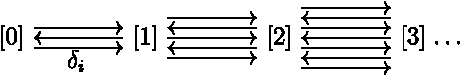
\includegraphics{delta_cat}
	\caption{The category $\DELTA$ with face and degeneracy maps.}
	\label{fig:delta_cat}
\end{figure}

Although this is a very abstract definition, a more geometric intuition can be given. In $\DELTA$ we can regard $[n]$ as an abstract version of the $n$-simplex $\Delta^n$. The face maps $\delta_i$ are then exactly maps which point out how we can embed $[n-1]$ in $[n]$. This is visualized in Figure~\ref{fig:delta_cat_geom}. This picture shows the images of the face maps, for example the image of $\delta_3$ from $[2]$ to $[3]$ is the set $\{0,1,2\}$, which corresponds to the bottom face of the tetrahedron. The degeneracy maps are harder to visualize, one can think of them as ``collapsing'' maps, where two points are identified with each other. For example, this collapses a triangle into a line.

\begin{figure}
	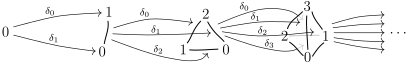
\includegraphics{delta_cat_geom}
	\caption{The category $\DELTA$ with the face maps shown in a geometric way.}
	\label{fig:delta_cat_geom}
\end{figure}

This category $\DELTA$ will act as a prototype for these kind of geometric structures in other categories. This leads to the following definition.

\begin{definition}
	A \emph{simplicial set} $X$ is a functor
	$$X: \DELTA^{op} \to \Set.$$
	(Or equivalently a contravariant functor $X: \DELTA \to \Set.$)
\end{definition}

The category $\sSet$ of all simplicial sets is the functor category $\Set^{\DELTA^{op}}$, where morphisms are natural transformations. Because the face and degeneracy maps give all the maps in $\DELTA$ it is sufficient to define images of $\delta_i$ and $\sigma_i$ in order to define a functor $X: \DELTA^{op} \to \Set$, keeping in mind that these should satisfy some relations which we will discuss next. Hence we can picture a simplicial set as done in Figure~\ref{fig:simplicial_set}. Comparing this to Figure~\ref{fig:delta_cat} we see that the arrows are reversed, because $X$ is a contravariant functor.

\begin{figure}
	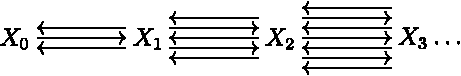
\includegraphics{simplicial_set}
	\caption{A simplicial set.}
	\label{fig:simplicial_set}
\end{figure}


\subsection{Explicit definition}
Of course the maps $\delta_i$ and $\sigma_i$ in $\DELTA$ satisfy certain relations, these are the so called \emph{cosimplicial identities}.

\begin{lemma}
	The face and degeneracy maps in $\DELTA$ satisfy the cosimplicial identities
	\begin{align}
		\delta_j\delta_i &= \delta_i\delta_{j-1},  \hspace{1.5cm} \textnormal{ if } i < j,\\
		\sigma_j\delta_i &= \delta_i\sigma_{j-1},  \hspace{1.5cm} \textnormal{ if } i < j,\\
		\sigma_j\delta_j &= \sigma_j\delta_{j+1} = \id,\\
		\sigma_j\delta_i &= \delta_{i-1}\sigma_j,  \hspace{1.5cm} \textnormal{ if } i > j+1,\\
		\sigma_j\sigma_i &= \sigma_i\sigma_{j+1},  \hspace{1.5cm} \textnormal{ if } i \leq j.
	\end{align}
\end{lemma}
\begin{proof}
	This follows immediately from the definitions.
\end{proof}

Note that these cosimplicial identities are ``purely categorical'', i.e. they only use compositions and identity maps. Because a simplicial set $X$ is a contravariant functor, dual versions of these equations hold in its image. For example, the first equation corresponds to $X(\delta_i)X(\delta_j) = X(\delta_{j-1})X(\delta_i)$ for $i < j$. This can be used for an explicit definition of simplicial sets. In this definition a simplicial set $X$ consists of a collection of sets $X_n$ together with face and degeneracy maps. More precisely:

\begin{lemma}
	A simplicial set $X$ is equivalently specified by a collection sets $X_n$, $n \in \N$, together with functions $d_i: X_n \to X_{n-1}$ and $s_i: X_n \to X_{n+1}$ for $0 \leq i \leq n$ and $n \in \N$, such that the simplicial identities hold
	\begin{align}
		d_i d_j &= d_{j-1} d_i,  \hspace{1.5cm} \text{ if } i < j,\\
		d_i s_j &= s_{j-1} d_i,  \hspace{1.5cm} \text{ if } i < j,\\
		d_j s_j &= d_{j+1} s_j = \id,\\
		d_i s_j &= s_j d_{i-1},  \hspace{1.5cm} \text{ if } i > j+1,\\
		s_i s_j &= s_{j+1} s_i,  \hspace{1.5cm} \text{ if } i \leq j.
	\end{align}
\end{lemma}

It is already indicated that a functor from $\DELTA^{op}$ to $\Set$ is determined when the images for the face and degeneracy maps in $\DELTA$ are provided. So this gives a way of restoring the definition from this specification. Conversely, we can apply functoriality to obtain this specification from the definition. We will not give the proof in more detail. From now on we will use the following notation for a simplicial set $X$:
$$ X_n = X([n]), \quad s_i = X(\sigma_i) \quad\text{and}\quad d_i = X(\delta_i). $$
For any other map $\beta : [n] \to [p]$ we will denote the induced map by $\beta^\ast: X_p \to X_n$.

When using a simplicial set to construct another object, it is often handy to use this second definition, as it gives you a very concrete objects to work with. On the other hand, constructing this might be hard (as you would need to provide a lot of details), in this case we will often use the more abstract definition.

Note that because of the third equation, the degeneracy maps $s_i$ are injective. This means that in the set $X_{n+1}$ there are always ``copies'' of elements of $X_n$. In a way these elements are not interesting, hence we call them degenerate.
\begin{definition}
	An element $x \in X_{n+1}$ is \emph{degenerate} if it lies in the image of $s_i: X_n \to X_{n+1}$ for some $i$, otherwise it is called \emph{non-degenerate}.
\end{definition}
\begin{lemma}
	\label{le:non-degenerate}
	We can write any $x \in X_n$ uniquely as $x = \beta^\ast y$ with $\beta: [n] \epi [m]$ a surjective map and $y \in X_m$ non-degenerate.
\end{lemma}
\begin{proof}
	We will proof the existence by induction over $n$. For $n=0$ the statement is trivial, since all elements in $X_0$ are non-degenerate. Assume the statement is proven for $n$. Let $x \in X_{n+1}$. Clearly if $x$ itself is non-degenerate, we can write $x = \id^\ast x$. Otherwise it is of the form $x = s_i x'$ for some $x' \in X_n$ and $i$. The induction hypothesis tells us that we can write $x' = \beta^\ast y$ for some surjection $\beta: [n] \epi [m]$ and $y \in X_m$ non-degenerate. So $x = s_i \beta^\ast y = (\beta \sigma_i)^\ast y$.

	For uniqueness, assume $x = \beta^\ast y = \gamma^\ast z$ with $\beta: [n] \epi [m]$, $\gamma: [n] \epi [m']$ and $y \in X_m, z \in X_{m'}$ non-degenerate. Because $\beta$ is surjective there is an $\alpha:[m]\to[n]$ such that $\beta\alpha = \id$ and hence $y = \alpha^\ast \beta^\ast y = \alpha^\ast \gamma^\ast z = (\gamma\alpha)^\ast z$. By the epi-mon factorization (Lemma~\ref{le:epimono}) we can write $\gamma\alpha = \delta_{i_a} \cdots \delta_{i_1} \sigma_{j_b} \cdots \sigma_{j_1}$, using that $y$ is non-degenerate we know that $\gamma\alpha$ is injective. So we have $\gamma\alpha: [m] \mono [m']$. Because of symmetry (of $y$ and $z$) we also have some map $[m'] \mono[m]$, so $m = m'$. So $\gamma\alpha$ is also surjective, hence the identity function, thus $y = z$, meaning that the non-degenerate $m$-simplex $y$ is unique.

	Now assume $x = \beta^\ast y = \gamma^\ast y$ with $\gamma, \beta: [n] \epi [m]$ such that $\beta \neq \gamma$, and $y \in X_m$ non-degenerate. Then we can find an $\alpha:[m]\to[n]$ such that $\beta\alpha = \id$ and $\gamma\alpha \neq \id$. With the epi-mono factorization write $\gamma\alpha = \delta_{i_a} \cdots \delta_{i_1} \sigma_{j_b} \cdots \sigma_{j_1}$, then by functoriality of $X$
	$$ y = \alpha^\ast \beta^\ast y = \alpha^\ast \gamma^\ast y = s_{j_1} \cdots s_{j_b} d_{i_1} \cdots d_{i_a} y. $$
	Note that $y$ was non-degenerate, so $s_{j_1} \cdots s_{j_b} = \id$, hence $d_{i_1} \cdots d_{i_a} = \id$. So $\gamma\alpha = \id$, which gives a contradiction. So $\beta = \gamma$, meaning that the surjection $\beta$ is also unique.
\end{proof}

\subsection{The standard $n$-simplex}
Recall that for any category $\cat{C}$ we have the $\mathbf{Hom}$-functor $\Hom{\cat{C}}{-}{-}: \cat{C}^{op} \times \cat{C} \to \Set$. We can fix an object $C \in \cat{C}$ and get a functor $\Hom{\cat{C}}{-}{C} : \cat{C}^{op} \to \Set$. In our case we can get the following simplicial sets in this way:

\begin{definition}
	The \emph{standard $n$-simplex} $\Delta[n] \in \sSet$ is given by
	$$\Delta[n] = \Hom{\DELTA}{-}{[n]} : \DELTA^{op} \to \Set.$$
\end{definition}

Note that $\Delta[-]: \DELTA \to \sSet$ is exactly the Yoneda embedding. So a $m$-simplex in $\Delta[n]$ is nothing more than a monotone function $[m] \to [n]$. In a moment we will see why the Yoneda lemma is useful to us, but let us first explicitly describe two examples of such standard simplices.

\begin{example}
	We will compute how $\Delta[0]$ look like. Note that $[0]$ is an one-element set, so for any set $S$, there is only one function $\ast: S \to [0]$. Hence $\Delta[0]_n = \{\ast\}$ for all $n$ and the face and degeneracy maps are necessarily the identity maps $\id: \{\ast\} \to \{\ast\}$. Thus, $\Delta[0]$ looks like
	$$ \Delta[0] :=
	\begin{tikzpicture}[baseline=-0.5ex]
	\matrix (m) [matrix of math nodes] { 
		\{\ast\} & \{\ast\} & \{\ast\} & \cdots \\
	}; 

	\foreach \r in {-5, 5} \draw [raise line=\r, <-] (m-1-1) -> (m-1-2);
	\foreach \r in {0} \draw [raise line=\r, ->] (m-1-1) -> (m-1-2);

	\foreach \r in {-10, 0, 10} \draw [raise line=\r, <-] (m-1-2) -> (m-1-3);
	\foreach \r in {-5, 5} \draw [raise line=\r, ->] (m-1-2) -> (m-1-3);

	\foreach \r in {-15, -5, 5, 15} \draw [raise line=\r, <-] (m-1-3) -> (m-1-4);
	\foreach \r in {-10, 0, 10} \draw [raise line=\r, ->] (m-1-3) -> (m-1-4);
	\end{tikzpicture}.$$
	Note that the only non-degenerate simplex is the unique $0$-simplex.
\end{example}

We can characterize the non-degenerate simplices for the other standard $n$-simplices as well. Recall that a simplex is degenerate if it lies the image of $s_i$ for some $i$. In the simplicial set $\Delta[n]$ the degeneracy maps $s_i$ are given by precomposing with $\sigma_i$ (by definition of the $\mathbf{Hom}$-functor). Given a $m$-simplex $x \in \Delta[n]_m$, using the epi-mono factorization we can write it as $x = \delta\sigma: [m] \to [n]$, where $\delta$ is injective and $\sigma$ surjective. It is now easily seen that $x$ is degenerate if and only if $\sigma \neq \id$. In other words a $m$-simplex $x \in \Delta[n]_m$ is non-degenerate if and only if $x: [m] \to [n]$ is injective. Note that for $m>n$ no such injective monotone functions exist and for $m=n$ there is a unique one, namely $\id_{[n]}$.

\begin{example}
	$\Delta[1]$ is a bit more interesting, but still not too complicated. We will describe the first three sets $\Delta[1]_0$, $\Delta[1]_1$ and $\Delta[1]_2$. We can use the fact that any monotone function $f: [n] \to [m]$ is a composition of first applying degeneracy maps, and then face maps, i.e.: $f: [n] \tot{\sigma_{i_0} \cdots \sigma_{i_M}} [k] \tot{\delta_{j_0} \cdots \delta_{j_N}} [m]$, where $k \leq m, n$.

	For $\Delta[1]_0$ we have to consider maps from $[0]$ to $[1]$, we cannot first apply degeneracy maps (there is no object $[-1]$). So this leaves us with the face maps: $\Delta[1]_0 = \{\delta_0, \delta_1\}$. For $\Delta[1]_1$ we of course have the identity function and two functions $\delta_0\sigma_0, \delta_1\sigma_0$. Now $\Delta[1]_2$ are the maps from $[2]$ to $[1]$.

	We will compute the two face maps $d_0$ and $d_1$ from $\Delta[1]_1$ to $\Delta[1]_0$. Recall that the $\mathbf{Hom}$-functor in the first argument (the contravariant argument) works with precomposition. So this gives
	\begin{align*}
		d_0(\id) &= \id \delta_0 = \delta_0 \\
		d_0(\delta_0\sigma_0) &= \delta_0 \sigma_0 \delta_0 = \delta_0 \\
		d_0(\delta_1\sigma_0) &= \delta_0 \sigma_0 \delta_0 = \delta_1.
	\end{align*}
	Where we in the first calculation used the identity law. In the second and third line we used the third simplicial equation, asserting that $\sigma_0 \delta_0 = \id$. Similarly we can calculate the face map $d_1$:
	\begin{align*}
		d_1(\id) &= \id \delta_1 = \delta_1 \\
		d_1(\delta_0\sigma_0) &= \delta_0 \sigma_0 \delta_1 = \delta_0 \\
		d_1(\delta_1\sigma_0) &= \delta_0 \sigma_0 \delta_1 = \delta_1.
	\end{align*}

	$$ \Delta[1] :=
	\begin{tikzpicture}[baseline=-0.5ex]
	\matrix (m) [matrix of math nodes] { 
		\{\delta_0, \delta_1\} & \{\delta_0 \sigma_0, \id, \delta_1 \sigma_0\} & \cdots \\
	}; 

	\foreach \r in {-5, 5} \draw [raise line=\r, <-] (m-1-1) -> (m-1-2);
	\foreach \r in {0} \draw [raise line=\r, ->] (m-1-1) -> (m-1-2);

	\foreach \r in {-10, 0, 10} \draw [raise line=\r, <-] (m-1-2) -> (m-1-3);
	\foreach \r in {-5, 5} \draw [raise line=\r, ->] (m-1-2) -> (m-1-3);

	\end{tikzpicture}.$$
	In this simplicial set there are three non-degenerate simplices. There is $\id \in \Delta[1]_1$, which clearly is non-degenerate, and the two $0$-simplices $\delta_0$ and $\delta_1$. One can think of this simplicial set as a line (the non-degenerate $1$-simplex) with its endpoints (the two $0$-simplices).
\end{example}

\subsection{Simplicial objects in arbitrary categories}
Of course the definition of simplicial set can easily be generalized to other categories. For any category $\cat{C}$ we can consider the functor category $\cat{sC} = \cat{C}^{\DELTA^{op}}$. In this thesis we are interested in the category of \emph{simplicial abelian groups}:
$$ \sAb = \Ab^{\DELTA^{op}}. $$
So a simplicial abelian group $A$ is a collection of abelian groups $A_n$, together with face and degeneracy maps, which in this case means group homomorphisms $d_i$ and $s_i$ such that the simplicial equations hold.

Note that the set of natural transformations between two simplicial abelian groups $A$ and $B$ is also an abelian group. The proof that $\sAb$ is a preadditive category is very similar to the proof we saw in Section~\ref{sec:Chain Complexes}. For two natural transformations $f,g: A \to B$ we simply define $f+g$ pointwise by $(f+g)_n = f_n + g_n$ and it is easily checked that this is a natural transformation.

As we are interested in simplicial abelian groups, it would be nice to obtain simplicial abelian groups associated to the standard $n$-simplices. We have seen how to make an abelian group out of any set using the free abelian group functor. We can use this functor $\Z[-]: \Set \to \Ab$ to induce a functor $\Z^\ast[-]: \sSet \to \sAb$ as shown in the following diagram.
\begin{figure}[h!]
	\begin{tikzpicture}
		\matrix (m) [matrix of math nodes]{
			\DELTA^{op} & \Set \\
			            & \Ab  \\
		};
		\path[->]
		(m-1-1) edge node[auto] {$ X $} (m-1-2)
		(m-1-2) edge node[auto] {$ \Z[-] $} (m-2-2)
		(m-1-1) edge node[below left] {$ \Z^\ast[X] $} (m-2-2);
	\end{tikzpicture}
	\caption{The simplicial set $X$ can be made into a simplicial abelian group $\Z^\ast[X]$ by postcomposing with $\Z[-]$.}
	\label{fig:diagram_Z}
\end{figure}
This construction obviously defines a functor $\Z^\ast[-] : \sSet \to \sAb$. Similarly, postcomposition with the forgetful functor $U: \Ab \to \Set$ gives rise to a forgetful functor $U^\ast: \sAb \to \sSet$. Thus in formulas we have
$$ \Z^\ast[X]_n = \Z[X_n] \quad\text{and}\quad U^\ast(A)_n = U(A_n). $$
This justifies that we may drop this extra decoration ($^\ast$) and write $\Z[-]$ (resp. $U$) instead of $\Z^\ast[-]$ (resp. $U^\ast$).

\begin{lemma}
	The functor $\Z[-]: \sSet \to \sAb$ is a left adjoint, with $U: \sAb \to \sSet$ as right adjoint.
\end{lemma}
As this is a purely categorical question (it even works for arbitrary functor categories), only a sketch of the proof is given. First note that by the fact that $\Z$ and $U$ already form an adjunction, and if we are given a natural transformation $f: X \to UA$ of simplicial sets we get the following diagram for each $n \in \N$:
\begin{center}
\begin{tikzpicture}
	\matrix (m) [matrix of math nodes]{
		X_n & U\Z[X]_n & \Z[X_n] \\
		    & U(A_n)   & A_n \\
	};
	\path[->]
	(m-1-1) edge node[auto] {$ \eta_{X_n} $} (m-1-2)
	(m-1-2) edge node[auto] {$ U(\overline{f}_n) $} (m-2-2)
	(m-1-1) edge node[auto] {$ f_n $} (m-2-2);
	\path[->]
	(m-1-3) edge node[auto] {$ \overline{f}_n $} (m-2-3);
\end{tikzpicture}
\end{center}
Then use naturality of $\eta$ (in $X_n$, thus in particular in $n$) to extend this to $\eta : X \to U\Z[X]$. The uniqueness of the maps $\overline{f}_n$ will assure that we get a natural transformation $\overline{f}: \Z[X] \to A$. The reader is invited to check the details.


\begin{example}
	We can apply this to the standard $n$-simplex $\Delta[1]$. This gives $\Delta[1]_0 \iso \Z^2$, since $\Delta[1]_0$ has two elements, and $\Z^\ast[\Delta[1]]_1 \iso \Z^3$, where the isomorphisms are taken such that
	\begin{align*}
		\delta_0         &\mapstot{\iso} (1, 0), \\
		\delta_1         &\mapstot{\iso} (0, 1), \\
		\delta_0\sigma_0 &\mapstot{\iso} (1, 0, 0), \\
		\id              &\mapstot{\iso} (0, 1, 0), \\
		\delta_1\sigma_0 &\mapstot{\iso} (0, 0, 1).
	\end{align*}
	The face maps from $\Z[\Delta[1]]_1$ to $\Z[\Delta[1]]_0$ under these isomorphisms are then given by
	\begin{align*}
		d_0(x, y, z) &= (x+y, z), \\
		d_1(x, y, z) &= (x, y+z).
	\end{align*}
\end{example}

\subsection{The Yoneda lemma}
Recall the statement of the Yoneda lemma from Section~\ref{sec:Category Theory}. In our case we consider functors $X: \DELTA^{op} \to \Set$ and objects $[n]$. So this gives us a natural bijection
$$ \Hom{\sSet}{\Delta[n]}{X} \iso X_n $$
telling us that we can regard $n$-simplices in $X$ as maps from $\Delta[n]$ to $X$. This also extends to the case of simplicial abelian groups.
\begin{lemma}\emph{(The additive Yoneda lemma)}
	Let $A$ be a simplicial abelian group. Then there is a group isomorphism
	$$ \Hom{\sAb}{\Z[\Delta[n]]}{A} \iso A_n, $$
	which is natural in $A$ and $[n]$.
\end{lemma}
\begin{proof}
	By using the (non-additive) Yoneda lemma and the fact that $\Z$ is a left adjoint, we already have a natural bijection:
	$$ \Hom{\sAb}{\Z[\Delta[n]]}{A} \iso \Hom{\sSet}{\Delta[n]}{U(A)} \iso U(A)_n = A_n. $$
	The only thing that we need to check is that this bijection preserves the group structure. Recall that this bijection from $\Hom{\sAb}{\Z[\Delta[n]]}{A}$ to $A_n$ is given by (where $\id = \id_{[n]}$ is a generator in $\Z[\Delta[n]]$)
	$$ \phi(f) = f_n(\id) \in X_n \quad\text{ for } f: \Delta[n] \to X. $$

	Now let $A$ be a simplicial abelian group and $f, g: \Z\Delta[n] \to A$ maps. Then we compute
	$$ \phi(f) + \phi(g) = f_n(\id) + g_n(\id) = (f_n + g_n)(\id) = (f+g)_n(\id) = \phi(f+g), $$
	where we regard $\id \in \Delta[n]$ as an element $\id \in \Z\Delta[n]$, we can do so by the unit of the adjunction. So this bijection is also a group homomorphism, hence we have an isomorphism $\Hom{\sAb}{\Z[\Delta[n]]}{A} \iso A_n$ of abelian groups.
\end{proof}
